\documentclass[11pt,a4paper]{article}

\usepackage[T1]{fontenc}
\usepackage[utf8]{inputenc}
\usepackage[portuges]{babel}
\usepackage[margin=2.4cm]{geometry}
\usepackage{booktabs}
\usepackage{graphicx}
\usepackage{amsmath}
\usepackage{listings}
\usepackage{xcolor}
\usepackage{caption}
\usepackage{float}
\usepackage{microtype}
\usepackage[hidelinks]{hyperref}

\newcommand{\valRazaoEvLoads}{1{,}0000}
\newcommand{\valRazaoEvMisses}{1{,}3050}
\newcommand{\valRazaoEvBrinst}{1{,}0000}
\newcommand{\valRazaoEvBrmiss}{1{,}0335}
\newcommand{\valFatUmPctErroP}{0{,}0033}
\newcommand{\valFatDoisPctAP}{0{,}0000}
\newcommand{\valFatDoisPctBP}{99{,}9965}
\newcommand{\valFatDoisPctABP}{0{,}0005}
\newcommand{\valFatDoisPctErroP}{0{,}0030}
\newcommand{\valFatDoisPvalA}{0{,}850}
\newcommand{\valFatDoisPvalAB}{0{,}0149}
\newcommand{\valPctTec}{50{,}96}
\newcommand{\valPctAloc}{43{,}94}
\newcommand{\valPctInter}{1{,}09}
\newcommand{\valPctResid}{4{,}00}
\newcommand{\valDesescalonado}{0}
\newcommand{\valTukeySignif}{24}
\newcommand{\valTukeyTotal}{28}
\newcommand{\valTPooled}{1{,}9935}
\newcommand{\valBrinstBase}{1{,}020}
\newcommand{\valTaxaCacheBase}{2{,}230}
\newcommand{\valTaxaBrBase}{0{,}1026}
\newcommand{\valBrinstInter}{1{,}018}
\newcommand{\valTaxaCacheInter}{0{,}019}
\newcommand{\valTaxaBrInter}{0{,}1021}
\newcommand{\valBrinstUnroll}{0{,}272}
\newcommand{\valTaxaCacheUnroll}{1{,}894}
\newcommand{\valTaxaBrUnroll}{0{,}3850}
\newcommand{\valBrinstTiling}{1{,}116}
\newcommand{\valTaxaCacheTiling}{0{,}012}
\newcommand{\valTaxaBrTiling}{1{,}5365}
\newcommand{\valDeltaLoads}{4{,}006}
\newcommand{\valDeltaLoadsAmp}{0{,}0007}
\newcommand{\valMissAbsEstBase}{650{,}0}
\newcommand{\valMissAbsDinBase}{136{,}3}
\newcommand{\valMissAbsEstInter}{3{,}6}
\newcommand{\valMissAbsDinInter}{3{,}5}
\newcommand{\valMissAbsEstUnroll}{457{,}9}
\newcommand{\valMissAbsDinUnroll}{176{,}6}
\newcommand{\valMissAbsEstTiling}{2{,}5}
\newcommand{\valMissAbsDinTiling}{2{,}5}
\newcommand{\valStrideLinha}{4.000}
\newcommand{\valPeriodoConjunto}{4.096}
\newcommand{\valLinhasPorConjunto}{15{,}6}
\newcommand{\valAssociatividade}{12}
\newcommand{\valBrinstPrevisto}{1{,}001}
\newcommand{\valBrinstPrevistoUnroll}{0{,}251}
\newcommand{\valTaxaCacheBaseEst}{3{,}812}
\newcommand{\valTaxaCacheBaseDin}{0{,}647}
\newcommand{\valLoadsBaseEst}{17{,}051}
\newcommand{\valLoadsBaseDin}{21{,}058}
\newcommand{\valMissesBaseEst}{650{,}0}
\newcommand{\valMissesBaseDin}{136{,}3}
\newcommand{\valFatUmShapiroP}{0{,}001268}
\newcommand{\valFatDoisShapiroP}{0{,}0384}
\newcommand{\valFatDoisFlignerLogitP}{0{,}409}
\newcommand{\valNMatriz}{1.000}
\newcommand{\valBloco}{32}
\newcommand{\valUnroll}{4}
\newcommand{\valReplicas}{10}
\newcommand{\valMedicoes}{80}
\newcommand{\valChecksum}{16.251.093.877.953}
\newcommand{\valTCelula}{2{,}2622}
\newcommand{\valCvTempoMin}{1{,}54}
\newcommand{\valCvTempoMax}{5{,}12}
\newcommand{\valCvLoadsMax}{0{,}0031}
\newcommand{\valCvBrinstMax}{0{,}1133}
\newcommand{\valRazaoAloc}{1{,}247}
\newcommand{\valGanhoEstBase}{1{,}00}
\newcommand{\valGanhoDinBase}{1{,}00}
\newcommand{\valGanhoEstInter}{1{,}36}
\newcommand{\valGanhoDinInter}{1{,}31}
\newcommand{\valGanhoEstTiling}{1{,}07}
\newcommand{\valGanhoDinTiling}{1{,}09}
\newcommand{\valGanhoEstUnroll}{0{,}96}
\newcommand{\valGanhoDinUnroll}{1{,}02}
\newcommand{\valFatUmPctA}{25{,}37}
\newcommand{\valFatUmPctB}{49{,}39}
\newcommand{\valFatUmPctAB}{25{,}24}
\newcommand{\valFatUmPctErro}{0{,}00}
\newcommand{\valFatUmPctLogA}{4{,}71}
\newcommand{\valFatUmPctLogB}{92{,}24}
\newcommand{\valFatUmPctLogAB}{2{,}96}
\newcommand{\valFatUmGlErro}{36}
\newcommand{\valFatUmAc}{-0{,}012}
\newcommand{\valFatUmDw}{1{,}995}
\newcommand{\valFatUmRazaoVar}{320{,}18}
\newcommand{\valFatUmPermMax}{0{,}0001}
\newcommand{\valFatUmPermConc}{3}
\newcommand{\valFatUmAlinhaMax}{0{,}168}
\newcommand{\valFatDoisPctA}{0{,}00}
\newcommand{\valFatDoisPctB}{100{,}00}
\newcommand{\valFatDoisPctAB}{0{,}00}
\newcommand{\valFatDoisPctErro}{0{,}00}
\newcommand{\valFatDoisPctLogA}{0{,}00}
\newcommand{\valFatDoisPctLogB}{100{,}00}
\newcommand{\valFatDoisPctLogAB}{0{,}00}
\newcommand{\valFatDoisGlErro}{36}
\newcommand{\valFatDoisAc}{0{,}059}
\newcommand{\valFatDoisDw}{1{,}876}
\newcommand{\valFatDoisRazaoVar}{37{,}73}
\newcommand{\valFatDoisPermMax}{0{,}8472}
\newcommand{\valFatDoisPermConc}{3}
\newcommand{\valFatDoisAlinhaMax}{0{,}276}


\captionsetup{font=small,labelfont=bf}
\setlength{\parskip}{0.45em}

\lstset{
  basicstyle=\ttfamily\footnotesize,
  keywordstyle=\color{blue!60!black},
  commentstyle=\color{gray},
  numbers=left, numberstyle=\tiny\color{gray},
  frame=single, rulecolor=\color{gray!40},
  breaklines=true, showstringspaces=false, tabsize=4,
  literate={á}{{\'a}}1 {é}{{\'e}}1 {í}{{\'i}}1 {ó}{{\'o}}1 {ú}{{\'u}}1
           {ã}{{\~a}}1 {õ}{{\~o}}1 {ç}{{\c c}}1 {â}{{\^a}}1 {ê}{{\^e}}1
}

\title{\vspace{-1.4cm}\textbf{Profiling de técnicas de otimização de código}\\[0.25em]
\large Planejamento fatorial $4\times2$ com \texttt{perf} sobre multiplicação de matrizes}
\author{}
\date{}

\begin{document}
\maketitle
\vspace{-2.2cm}

\begin{center}
\begin{tabular}{@{}ll@{}}
\toprule
\textbf{Disciplina} & SSC0951 - Desenvolvimento de Código Otimizado \\
\textbf{Docente}    & Hermes Senger \\
\textbf{Alunos}     & Samuel Rubens Souza Oliveira (NUSP 11912533) \\
                    & José Guilherme Santos Riberto (NUSP 15647503) \\
\textbf{Atividade}  & Relativa à aula 3 (Profiling) \\
\bottomrule
\end{tabular}
\end{center}

\section{Enunciado da atividade}

O objetivo é o estudo das técnicas de otimização de código apresentadas na aula 3,
Loop Interchange e Loop Unrolling, utilizando o perfilador \texttt{perf} e técnicas de
análise de resultados. A configuração dos experimentos é fixada pelo enunciado.

\textbf{Fator 1, técnica de otimização de código}, com quatro níveis: sem otimização,
Loop Interchange, Loop Unrolling e Loop Tiling.

\textbf{Fator 2, alocação da matriz na memória}, com dois níveis: estática e dinâmica.

\begin{sloppypar}
\textbf{Métricas a coletar} em cada experimento: tempo de resposta,
\texttt{L1-dcache-loads}, \texttt{L1-dcache-load-misses}, \texttt{branch-instructions}
e \texttt{branch-misses}.
\end{sloppypar}

O cruzamento dos dois fatores define oito experimentos, numerados de 1 a 8 conforme a
Tabela~\ref{tab:mapa}. Cada experimento deve ser executado pelo menos dez vezes, e
deve-se calcular a média e o intervalo de confiança a 95\% das métricas coletadas.

\subsection*{As duas análises pedidas}

O enunciado encerra especificando duas análises, que são as perguntas que este relatório
responde de forma objetiva nas Seções~\ref{sec:analise1} e~\ref{sec:analise2}.

\begin{enumerate}
  \item \textbf{Comparação do tempo de resposta nos 8 experimentos.}
  \item \textbf{Influência da variação dos fatores nas variáveis de resposta de cache},
  considerando os experimentos 1, 2 e outros dois com a mesma técnica, à escolha entre
  [3 e 4], [5 e 6] ou [7 e 8], \textbf{e influência da variação dos fatores nas
  variáveis de resposta de branch}, considerando os experimentos 1, 2 e outros dois com
  a mesma técnica, também à escolha.
\end{enumerate}

Para a análise de cache foram escolhidos os experimentos \textbf{1, 2, 3 e 4}, ou seja
Loop Interchange, porque é a técnica que atua diretamente sobre o padrão de acesso à
memória. Para a análise de branch foram escolhidos os experimentos
\textbf{1, 2, 5 e 6}, ou seja Loop Unrolling, porque é a técnica que atua diretamente
sobre o controle de laço e portanto sobre a contagem de desvios.

\section{Descrição da atividade realizada}

\subsection{Programa medido}

O programa é a multiplicação de matrizes quadradas densas $C = A \cdot B$ com
$N = \valNMatriz$ e elementos do tipo \texttt{int}. As três matrizes ocupam
11,44~MiB no total, valor muito acima da cache L3 de 12~MiB desta máquina, de
modo que o padrão de acesso à memória é o fator dominante de desempenho e as técnicas
sob estudo têm efeito mensurável.

Os oito binários correspondem exatamente às oito células do planejamento.

\begin{table}[H]
\centering
\caption{Mapeamento dos oito experimentos do enunciado para os binários medidos.}
\label{tab:mapa}
\small
\begin{tabular}{@{}clll@{}}
\toprule
\textbf{Exp.} & \textbf{Técnica} & \textbf{Alocação} & \textbf{Kernel executado} \\
\midrule
1 & sem otimização   & estática & \texttt{multiplyMatrixStatic} \\
2 & sem otimização   & dinâmica & \texttt{multiplyMatrix} \\
3 & Loop Interchange & estática & \texttt{loopInterchangeMultStatic} \\
4 & Loop Interchange & dinâmica & \texttt{loopInterchangeMult} \\
5 & Loop Unrolling   & estática & \texttt{loopUnrollingMultStatic} \\
6 & Loop Unrolling   & dinâmica & \texttt{loopUnrollingMult} \\
7 & Loop Tiling      & estática & \texttt{loopTilingMultStatic} \\
8 & Loop Tiling      & dinâmica & \texttt{loopTilingMult} \\
\bottomrule
\end{tabular}
\end{table}

\subsection{Os quatro níveis do Fator 1}

Cada nível aplica \textbf{uma única} transformação sobre o mesmo laço base. Essa
disciplina é necessária para que o efeito principal da técnica seja atribuível: se um
nível carregasse duas transformações ao mesmo tempo, o efeito e a interação ficariam
confundidos.

\begin{itemize}
  \item \textbf{Sem otimização}: ordem $i$-$j$-$k$. O laço interno percorre uma linha de
  $A$ e uma \emph{coluna} de $B$, com passo de \valStrideLinha~bytes.
  \item \textbf{Loop Interchange}: única mudança é trocar $j$ e $k$, resultando em
  $i$-$k$-$j$. O laço interno passa a percorrer uma linha de $B$ e uma linha de $C$,
  ambas sequenciais, e \texttt{a[i][k]} fica invariante.
  \item \textbf{Loop Unrolling}: mantém a ordem $i$-$j$-$k$ da base e desenrola o laço
  mais interno em \valUnroll{} cópias, com laço de resto para correção em qualquer $N$.
  \item \textbf{Loop Tiling}: bloqueia o espaço de iteração em cubos de lado
  \valBloco, mantendo a ordem interna $i$-$j$-$k$ \emph{idêntica} à base. O lado
  \valBloco{} foi escolhido a partir da geometria da L1d, conforme a
  Seção~\ref{sec:bloco}.
\end{itemize}

\subsection{Os dois níveis do Fator 2}

Na alocação \textbf{estática} as matrizes são arrays de tamanho fixo e contíguos,
declarados em escopo de arquivo. O escopo de arquivo é obrigatório e não estilístico:
11,44~MiB excedem o limite de pilha de 8~MiB desta máquina, e em \texttt{-O0} o
compilador não emite verificação de pilha, de modo que o estouro seria uma falha de
segmentação sem diagnóstico.

Na alocação \textbf{dinâmica} as matrizes são \texttt{int**} com uma chamada de
\texttt{malloc} por linha, portanto as linhas não são contíguas entre si.

Os quatro laços da família estática são \emph{idênticos caractere por caractere} aos da
família dinâmica. A única diferença entre as duas famílias é o tipo do parâmetro,
\texttt{int m[N][N]} contra \texttt{int **m}, e portanto o endereçamento. Essa
equivalência foi verificada por comparação automática do texto dos kernels.

A escolha de passar as matrizes como \textbf{parâmetro} em ambas as famílias, em vez de
deixar o kernel estático ler diretamente variáveis globais, é o que mantém a comparação
honesta. Em \texttt{-O0}, uma leitura de elemento custa três loads na forma
\texttt{int **m}, dois na forma \texttt{int m[N][N]} e apenas um se o kernel lesse um
global. A diferença real entre as duas alocações é um load de ponteiro dependente mais a
perda de contiguidade entre linhas. A forma de parâmetro captura exatamente isso. A
forma global adicionaria uma segunda unidade de diferença, que é artefato de passagem de
parâmetro e não de alocação, e inflaria artificialmente o efeito do Fator 2 na métrica
de loads.

\subsection{Escolha do lado do bloco do Loop Tiling}
\label{sec:bloco}

A L1d desta máquina tem 48~KiB, linha de 64~bytes e \valAssociatividade{} vias. O
orçamento ingênuo, exigindo que três blocos de \texttt{int} caibam em 48~KiB, permitiria
lado até 64. Esse cálculo está errado porque as linhas da matriz distam
\valStrideLinha~bytes e nunca ficam alinhadas em 64~bytes, de modo que uma linha de
bloco de $T$ inteiros ocupa $\lceil (4T+63)/64 \rceil$ linhas de cache. Com $T = 64$ o
pior caso chega a 60~KiB e estoura a L1d. Com $T = \valBloco$ o pior caso é 18,0~KiB, ou
37\% da L1d, deixando folga para a pilha e para o carregamento do bloco seguinte.

O lado \valBloco{} também tem a vantagem de que $\valNMatriz \bmod \valBloco = 8$,
portanto o último bloco de cada dimensão tem largura 8 e as guardas de resto são
executadas em toda execução. Um lado que dividisse $N$ exatamente tornaria essas guardas
código morto, nunca exercitado, embora continuassem necessárias para correção.

\subsection{Protocolo de medição}

Todos os oito binários são compilados com o mesmo comando, sem qualquer otimização:
\texttt{gcc -O0 -std=c11 -Wall -Wextra -Werror}. A ausência de \texttt{-O} é exigida pelo
enunciado e é estrutural: em \texttt{-O0} o compilador não vetoriza nem aplica
transformação de laço, portanto as quatro variantes escritas à mão são genuinamente o que
se mede. O Fator 1 é o código fonte, não o compilador.

O tempo de resposta é medido com \texttt{clock\_gettime(CLOCK\_MONOTONIC)} imediatamente
antes e depois da chamada do kernel, e é registrado em nanossegundos inteiros. O
preenchimento das matrizes de entrada e a zeragem de $C$ acontecem \emph{antes} do
relógio, e os quatro kernels não zeram $C$. Isso mantém fora da região cronometrada tanto
o custo do gerador pseudoaleatório quanto as faltas de página de primeiro toque, cujo
custo difere entre as duas famílias de alocação e seria atribuído ao Fator 2 pelo motivo
errado.

Os quatro contadores são coletados com \texttt{perf stat} envolvendo o processo. Foram
adotadas as seguintes medidas de controle de variabilidade:

\begin{itemize}
  \item execuções fixadas em um núcleo de desempenho com \texttt{taskset -c 0}
  \item uma execução de aquecimento por célula, descartada
  \item ordem de execução das \valMedicoes{} medições \textbf{randomizada} com semente
  fixa e persistida em arquivo, o que protege os efeitos dos fatores de se confundirem
  com deriva térmica progressiva
  \item \valReplicas{} réplicas por célula, atendendo ao mínimo de dez do enunciado.
\end{itemize}

Duas observações são necessárias para interpretar corretamente os números que seguem.

\textbf{As oito variantes calculam o mesmo produto.} Isso foi verificado de duas formas
independentes, e é o que torna a comparação entre células legítima. O
Apêndice~\ref{ap:validade} traz o procedimento.

\textbf{O evento \texttt{L1-dcache-load-misses} mede algo mais amplo que apenas misses
de load de demanda} nesta máquina, por fator \valRazaoEvMisses{} em relação ao evento
nativo equivalente. Como o mesmo evento foi usado em todas as \valMedicoes{} medições, as
comparações entre células permanecem válidas, mas o valor absoluto não deve ser lido como
taxa de miss de demanda. O Apêndice~\ref{ap:eventos} detalha a verificação.

\section{Análise 1: comparação do tempo de resposta}
\label{sec:analise1}

A Tabela~\ref{tab:tempo} traz a média e o intervalo de confiança a 95\% do tempo de
resposta nos oito experimentos. O intervalo é o intervalo $t$ por célula,
$\bar{x} \pm t_{0{,}975} \cdot s/\sqrt{\valReplicas}$, com \valReplicas{} réplicas,
9 graus de liberdade e $t_{0{,}975} = \valTCelula$. Essa escolha atende ao enunciado, que pede intervalo para cada métrica
em \emph{cada} experimento. Um intervalo com erro quadrático médio agrupado seria mais
estreito, porém válido apenas sob homocedasticidade, pressuposto que a
Seção~\ref{sec:pressupostos} rejeita.

\begin{table}[H]
\centering
\caption{Tempo de resposta do kernel, em milissegundos. Média, semiamplitude do
intervalo de confiança a 95\%, limites do intervalo e coeficiente de variação.}
\label{tab:tempo}
\small
\begin{tabular}{@{}cllrrrrr@{}}
\toprule
\textbf{Exp.} & \textbf{Técnica} & \textbf{Alocação} & \textbf{Média} &
\textbf{$\pm$ IC} & \textbf{IC inf.} & \textbf{IC sup.} & \textbf{CV (\%)} \\
\midrule
1 & base & estatica & $4.319{,}4$ & $71{,}0$ & $4.248{,}4$ & $4.390{,}4$ & $2{,}30$ \\
2 & base & dinamica & $5.469{,}0$ & $200{,}1$ & $5.268{,}8$ & $5.669{,}1$ & $5{,}12$ \\
3 & interchange & estatica & $3.180{,}5$ & $35{,}0$ & $3.145{,}5$ & $3.215{,}5$ & $1{,}54$ \\
4 & interchange & dinamica & $4.173{,}8$ & $139{,}3$ & $4.034{,}5$ & $4.313{,}2$ & $4{,}67$ \\
5 & unrolling & estatica & $4.509{,}8$ & $130{,}9$ & $4.378{,}9$ & $4.640{,}8$ & $4{,}06$ \\
6 & unrolling & dinamica & $5.364{,}8$ & $167{,}0$ & $5.197{,}8$ & $5.531{,}7$ & $4{,}35$ \\
7 & tiling & estatica & $4.052{,}4$ & $69{,}1$ & $3.983{,}3$ & $4.121{,}6$ & $2{,}39$ \\
8 & tiling & dinamica & $5.021{,}3$ & $103{,}5$ & $4.917{,}8$ & $5.124{,}8$ & $2{,}88$
\\
\bottomrule
\end{tabular}
\end{table}

A Figura~\ref{fig:tempo} apresenta a mesma informação graficamente, com as barras de erro
do intervalo de confiança. Os experimentos aparecem na ordem do enunciado e não ordenados
por valor, para que a estrutura do planejamento permaneça legível.

\begin{figure}[H]
\centering
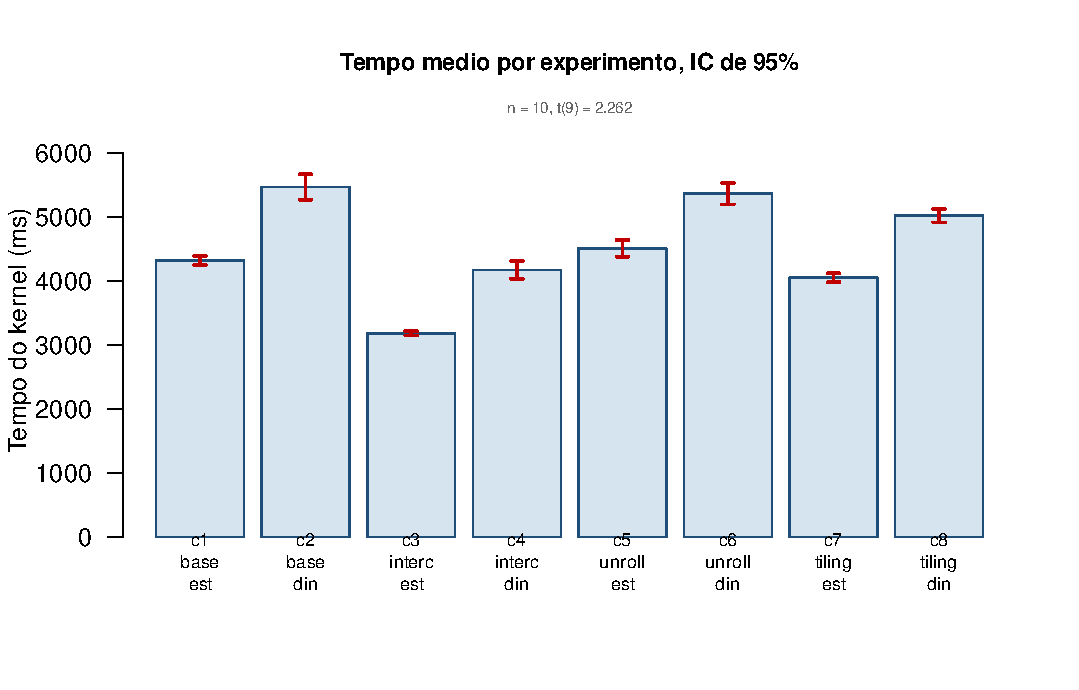
\includegraphics[width=0.92\textwidth]{figuras/tempo_barras.pdf}
\caption{Tempo médio de resposta nos oito experimentos, com barras de erro do intervalo
de confiança a 95\%.}
\label{fig:tempo}
\end{figure}

\begin{figure}[H]
\centering
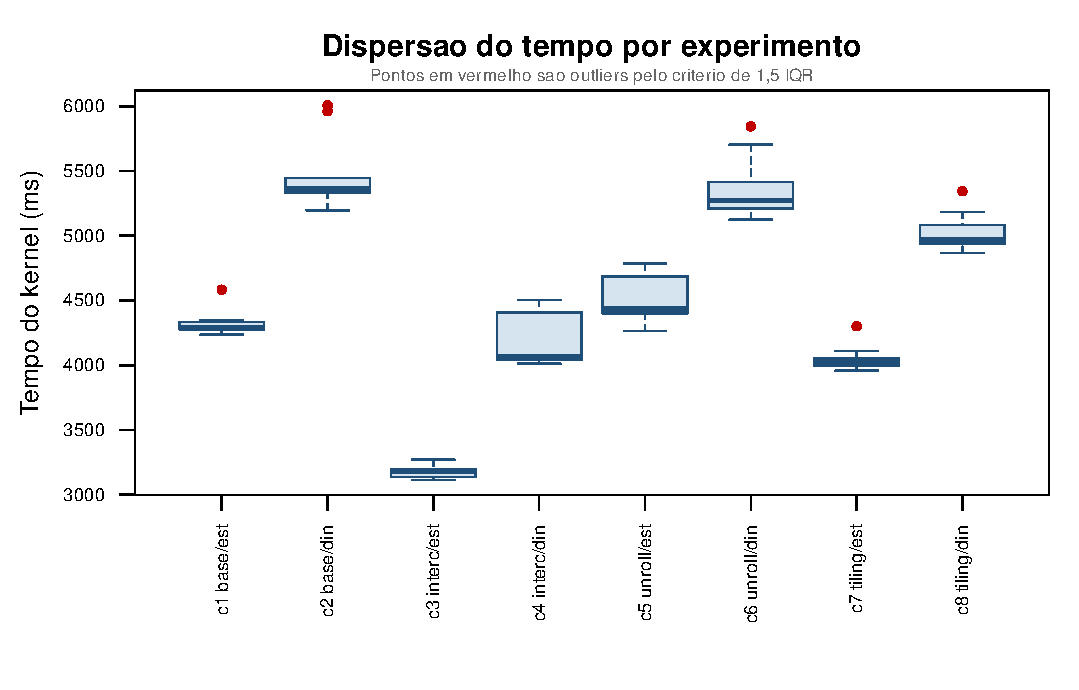
\includegraphics[width=0.86\textwidth]{figuras/boxplot_tempo.pdf}
\caption{Dispersão do tempo de resposta por experimento. Os pontos em vermelho são
valores atípicos pelo critério de 1,5 vez a amplitude interquartil.}
\label{fig:boxplot}
\end{figure}

\subsection{Leitura dos resultados}

O coeficiente de variação do tempo ficou entre \valCvTempoMin\% e \valCvTempoMax\%.
As comparações par a par de Tukey, com correção para as \valTukeyTotal{} comparações
possíveis, apontam \valTukeySignif{} pares significativos a 5\%, o que legitima a leitura
direta das diferenças no gráfico de barras.

Três resultados se destacam.

\textbf{Loop Interchange é a técnica mais eficaz}, com ganho de \valGanhoEstInter$\times$
na alocação estática e \valGanhoDinInter$\times$ na dinâmica sobre o caso sem otimização.
O motivo é direto: trocar $j$ e $k$ elimina o passeio por coluna de $B$, substituindo um
acesso com passo de \valStrideLinha~bytes por um acesso sequencial.

\textbf{Loop Tiling rende bem menos}, \valGanhoEstTiling$\times$ e
\valGanhoDinTiling$\times$. Isso é coerente com o fato de que o bloqueio foi aplicado
sobre a ordem $i$-$j$-$k$ da base, mantendo o passeio por coluna dentro de cada bloco. O
bloqueio reduz o alcance desse passeio, mas não o elimina como o interchange faz.

\textbf{Loop Unrolling não acelera, e na alocação estática chega a atrasar},
\valGanhoEstUnroll$\times$ contra a base. O resultado não é defeito de implementação: a
contagem de instruções de branch caiu de \valBrinstBase$\times10^9$ para
\valBrinstUnroll$\times10^9$, ou seja o desenrolamento de fator \valUnroll{} funcionou
exatamente como pretendido. O que ocorre é que, em \texttt{-O0}, o custo dos recálculos
de endereço para $k+1$, $k+2$ e $k+3$ supera a economia de controle de laço. A
transformação reduz desvios sem reduzir tempo.

Quanto ao Fator 2, a alocação dinâmica é em média \valRazaoAloc$\times$ mais lenta que a
estática, e essa ordenação se mantém em todas as quatro técnicas.

\section{Análise 2: influência dos fatores nas variáveis de cache e de branch}
\label{sec:analise2}

Esta seção responde a segunda pergunta do enunciado. São dois planejamentos $2\times2$
independentes em resposta, cada um com \valReplicas{} réplicas por célula, portanto 40
observações e \valFatUmGlErro{} graus de liberdade de erro.

A codificação dos contrastes é $x_A = -1$ para alocação estática e $+1$ para dinâmica, e
$x_B = -1$ para o caso sem otimização e $+1$ para a técnica sob teste. O modelo é
\begin{equation}
y = q_0 + q_A x_A + q_B x_B + q_{AB} x_A x_B + e,
\end{equation}
e a variação atribuída a cada efeito é $SS_i = 2^2 \cdot r \cdot q_i^2$.

Os efeitos foram calculados por dois caminhos independentes, a matriz de sinais e a
análise de variância, e verificou-se por código que as somas de quadrados coincidem. Uma
terceira rota, pelas médias marginais, reproduz $SS_A$ e $SS_B$. Três caminhos
concordantes constituem prova, enquanto um caminho isolado seria apenas afirmação.

\subsection{Média e intervalo de confiança dos contadores}

O enunciado exige média e intervalo de confiança para todas as métricas coletadas. A
Tabela~\ref{tab:contadores} traz os quatro contadores nos oito experimentos.

\begin{table}[H]
\centering
\caption{Contadores de hardware nos oito experimentos, média e semiamplitude do intervalo
de confiança a 95\%. Loads e instruções de branch em $10^9$, misses em $10^6$.}
\label{tab:contadores}
\scriptsize
\begin{tabular}{@{}cllrrrr@{}}
\toprule
\textbf{Exp.} & \textbf{Técnica} & \textbf{Aloc.} & \textbf{L1d loads ($10^9$)} &
\textbf{L1d misses ($10^6$)} & \textbf{br. inst. ($10^9$)} &
\textbf{br. misses ($10^6$)} \\
\midrule
1 & base & estatica & $17{,}051$ $\pm$ $0{,}0002$ & $649{,}96$ $\pm$ $1{,}03$ & $1{,}019$ $\pm$ $0{,}0001$ & $1{,}042$ $\pm$ $0{,}002$ \\
2 & base & dinamica & $21{,}058$ $\pm$ $0{,}0005$ & $136{,}30$ $\pm$ $2{,}53$ & $1{,}021$ $\pm$ $0{,}0003$ & $1{,}051$ $\pm$ $0{,}003$ \\
3 & interchange & estatica & $17{,}049$ $\pm$ $0{,}0001$ & $3{,}55$ $\pm$ $0{,}31$ & $1{,}018$ $\pm$ $0{,}0000$ & $1{,}037$ $\pm$ $0{,}001$ \\
4 & interchange & dinamica & $21{,}055$ $\pm$ $0{,}0003$ & $3{,}54$ $\pm$ $0{,}14$ & $1{,}019$ $\pm$ $0{,}0002$ & $1{,}043$ $\pm$ $0{,}003$ \\
5 & unrolling & estatica & $15{,}803$ $\pm$ $0{,}0003$ & $457{,}90$ $\pm$ $1{,}24$ & $0{,}271$ $\pm$ $0{,}0002$ & $1{,}046$ $\pm$ $0{,}003$ \\
6 & unrolling & dinamica & $19{,}810$ $\pm$ $0{,}0003$ & $176{,}55$ $\pm$ $2{,}17$ & $0{,}273$ $\pm$ $0{,}0002$ & $1{,}049$ $\pm$ $0{,}002$ \\
7 & tiling & estatica & $18{,}246$ $\pm$ $0{,}0001$ & $2{,}50$ $\pm$ $0{,}04$ & $1{,}115$ $\pm$ $0{,}0001$ & $32{,}080$ $\pm$ $0{,}003$ \\
8 & tiling & dinamica & $22{,}252$ $\pm$ $0{,}0002$ & $2{,}51$ $\pm$ $0{,}05$ & $1{,}116$ $\pm$ $0{,}0002$ & $2{,}182$ $\pm$ $0{,}097$
\\
\bottomrule
\end{tabular}
\end{table}

\begin{figure}[H]
\centering
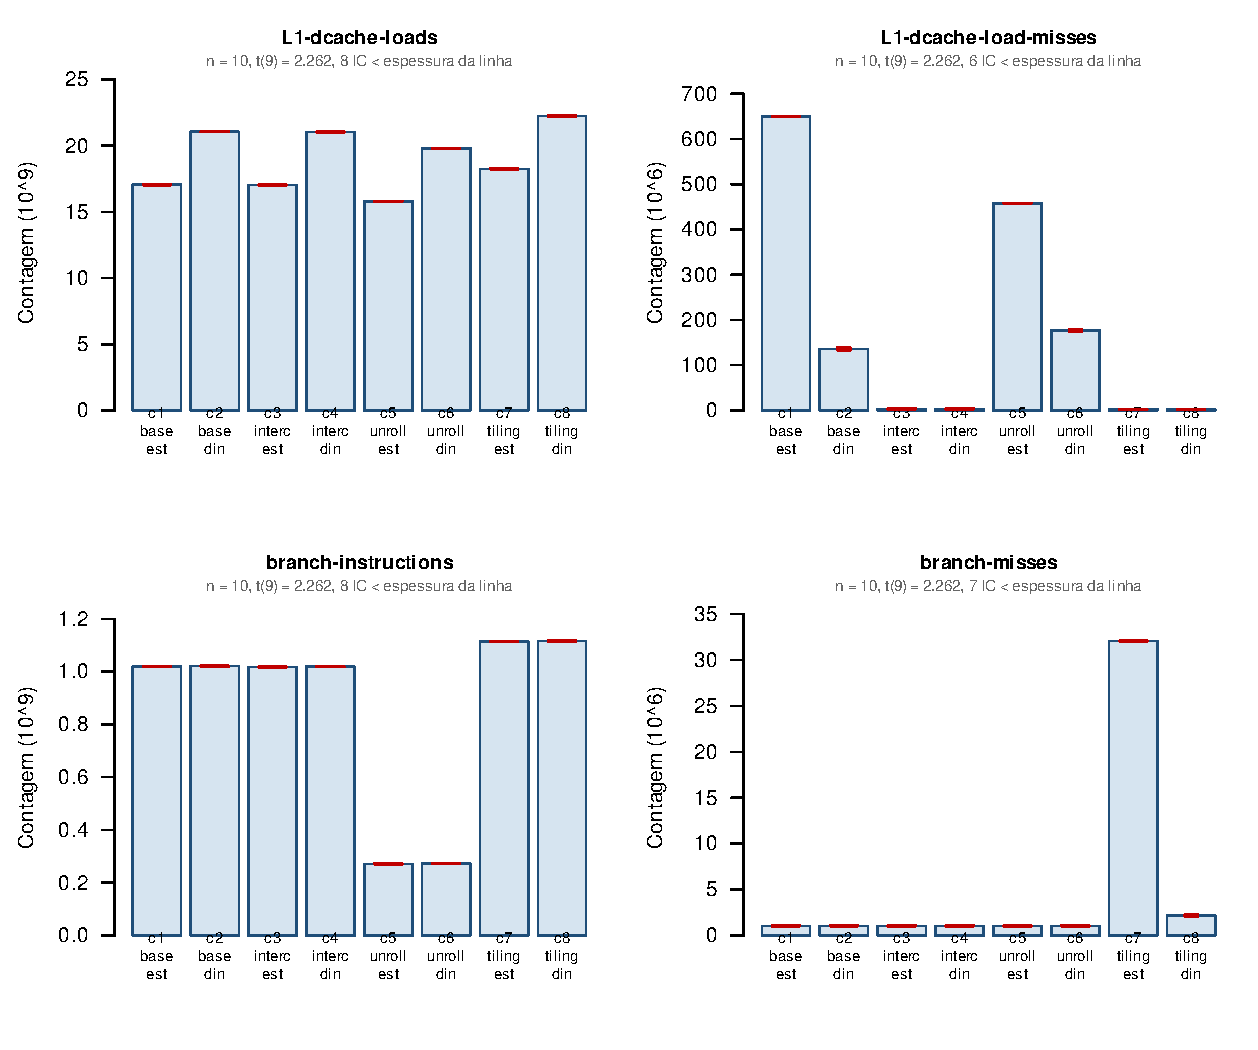
\includegraphics[width=0.98\textwidth]{figuras/contadores_barras.pdf}
\caption{Os quatro contadores de hardware nos oito experimentos, com intervalo de
confiança a 95\%. Nos contadores de loads e de instruções de branch o intervalo é mais
estreito que a espessura da linha, o que é informação e não defeito: essas duas métricas
são função quase determinística do fluxo de instruções executado.}
\label{fig:contadores}
\end{figure}

\begin{sloppypar}
Uma observação metodológica decorre da Figura~\ref{fig:contadores}. O coeficiente de
variação de \texttt{L1-dcache-loads} não passa de \valCvLoadsMax\% e o de
\texttt{branch-instructions} não passa de \valCvBrinstMax\%, ou seja essas duas métricas
são essencialmente determinísticas. O erro quadrático médio das análises que as envolvem
fica minúsculo, os valores de $F$ ficam enormes e quase todo $p$ resulta inferior a
$2\times10^{-16}$. \textbf{A significância estatística passa a ser garantida e portanto
não informativa}, e o que interpreta este experimento é o tamanho do efeito e a alocação
percentual de variação. A Seção~\ref{sec:fat2} traz um caso concreto disso.
\end{sloppypar}

\subsection{Análise de cache: experimentos 1, 2, 3 e 4}

A variável de resposta é a \textbf{taxa de miss de L1d}, definida como
\texttt{L1-dcache-load-misses} dividido por \texttt{L1-dcache-loads}. A taxa é preferível
à contagem absoluta como resposta do planejamento porque é adimensional, mas a
Seção~\ref{sec:absoluto} mostra que as duas leituras precisam ser apresentadas juntas.

\begin{table}[H]
\centering
\caption{Alocação de variação e coeficientes do modelo, análise de cache sobre a taxa de
miss de L1d, experimentos 1 a 4.}
\label{tab:fat1}
\small
\begin{tabular}{@{}lrrrr@{}}
\toprule
\textbf{Fonte} & \textbf{SS} & \textbf{Influência (\%)} & \textbf{$q$} & \textbf{$p$} \\
\midrule
$A$ (aloca\c{c}\~ao) & $0{,}002510$ & $25{,}3670$ & $-0{,}007922$ & $<2\times10^{-16}$ \\
$B$ (interchange) & $0{,}004887$ & $49{,}3919$ & $-0{,}01105$ & $<2\times10^{-16}$ \\
$AB$ (intera\c{c}\~ao) & $0{,}002497$ & $25{,}2378$ & $0{,}007901$ & $<2\times10^{-16}$ \\
Erro & $3{,}241\times10^{-7}$ & $0{,}0033$ & -- & --
\\
\bottomrule
\end{tabular}
\end{table}

\begin{table}[H]
\centering
\caption{Análise de variância, análise de cache.}
\label{tab:anova1}
\small
\begin{tabular}{@{}lrrrrr@{}}
\toprule
\textbf{Fonte} & \textbf{gl} & \textbf{SS} & \textbf{MS} & \textbf{$F$} & \textbf{$p$} \\
\midrule
$A$ (aloca\c{c}\~ao) & 1 & $0{,}002510$ & $0{,}002510$ & $2{,}788\times10^{5}$ & $<2\times10^{-16}$ \\
$B$ (interchange) & 1 & $0{,}004887$ & $0{,}004887$ & $5{,}429\times10^{5}$ & $<2\times10^{-16}$ \\
$AB$ (intera\c{c}\~ao) & 1 & $0{,}002497$ & $0{,}002497$ & $2{,}774\times10^{5}$ & $<2\times10^{-16}$ \\
Res\'iduos & 36 & $3{,}241\times10^{-7}$ & $9{,}002\times10^{-9}$ & -- & --
\\
\bottomrule
\end{tabular}
\end{table}

\begin{figure}[H]
\centering
\begin{minipage}{0.49\textwidth}
\centering
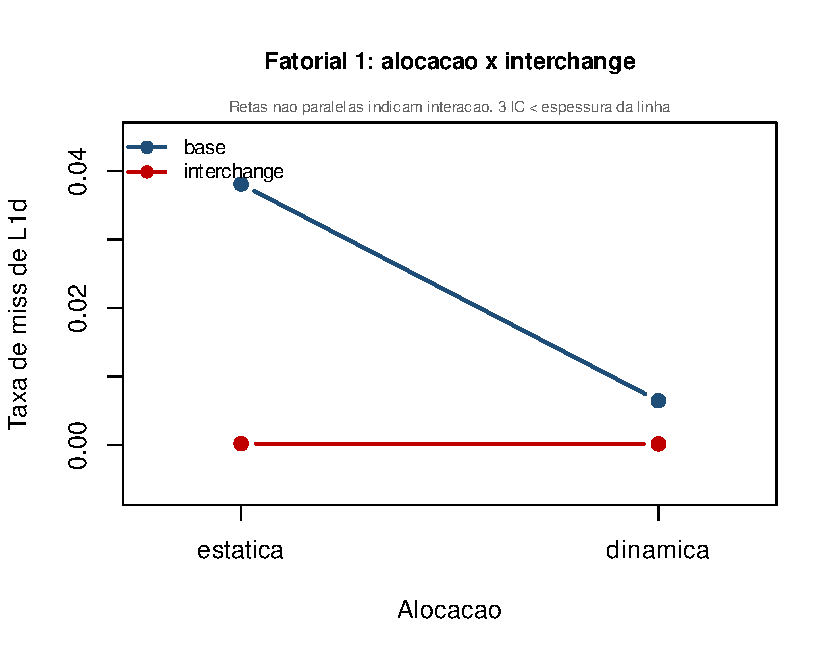
\includegraphics[width=\textwidth]{figuras/interacao_fat1.pdf}
\end{minipage}
\begin{minipage}{0.49\textwidth}
\centering
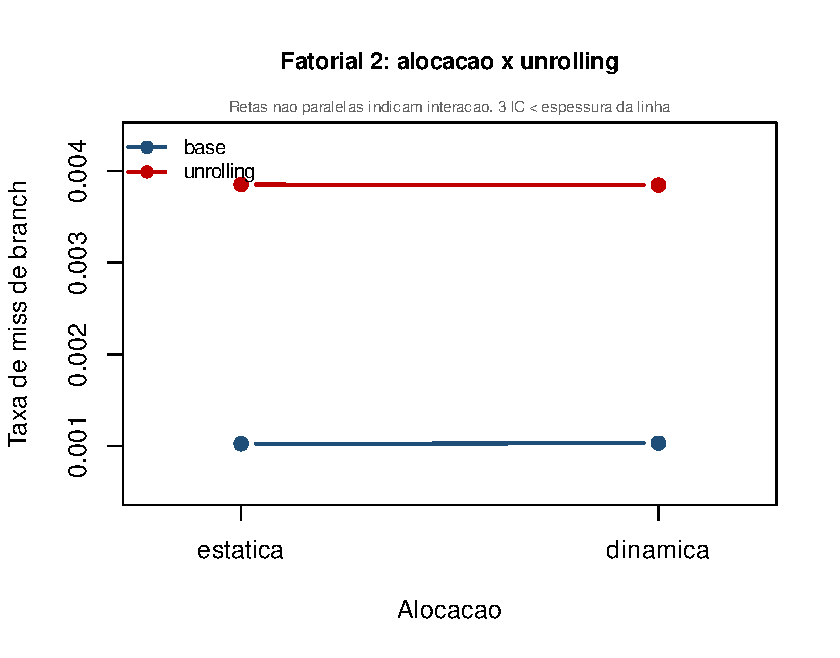
\includegraphics[width=\textwidth]{figuras/interacao_fat2.pdf}
\end{minipage}
\caption{Gráficos de interação. À esquerda a análise de cache, à direita a de branch.
Retas não paralelas indicam interação entre os fatores.}
\label{fig:interacao}
\end{figure}

O resultado central é que os três termos têm influência da mesma ordem de grandeza:
a técnica responde por \valFatUmPctB\%, a alocação por \valFatUmPctA\% e a
\textbf{interação por \valFatUmPctAB\%}. O erro fica em \valFatUmPctErroP\%.

Uma interação que responde por um quarto da variação é o achado mais relevante desta
análise, e o gráfico de interação da Figura~\ref{fig:interacao} explica o mecanismo. No
kernel sem otimização, a taxa de miss cai de \valTaxaCacheBaseEst\% na alocação estática
para \valTaxaCacheBaseDin\% na dinâmica, uma diferença grande. No kernel com interchange,
as duas alocações ficam praticamente empatadas, em torno de \valTaxaCacheInter\%.

Em outras palavras, \textbf{a alocação só importa enquanto existe o passeio por coluna}.
O Loop Interchange elimina esse passeio, e ao fazê-lo torna a escolha da alocação
irrelevante para a cache. Esse é o tipo exato de conclusão que um experimento de um fator
por vez não produziria: variando apenas a alocação com o kernel base, concluir-se-ia que
a alocação tem forte influência sobre a cache, o que é falso para três das quatro
técnicas.

\begin{figure}[H]
\centering
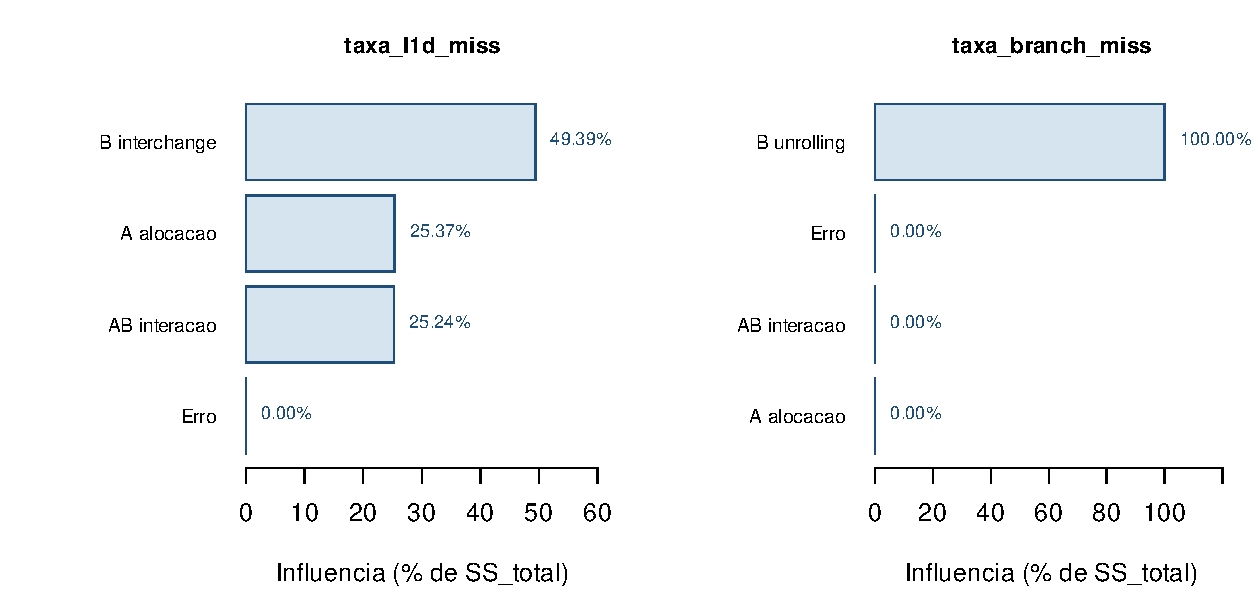
\includegraphics[width=0.94\textwidth]{figuras/pareto_influencia.pdf}
\caption{Influência percentual de cada termo nas duas análises. À esquerda a resposta de
cache, à direita a de branch. Os quatro valores de cada painel somam 100\%.}
\label{fig:pareto}
\end{figure}

\subsection{Contagem absoluta contra taxa}
\label{sec:absoluto}

A taxa de miss e a contagem absoluta de misses apontam em direções diferentes neste
experimento, e apresentar apenas uma das duas seria enganoso.

O denominador da taxa depende da alocação. A família dinâmica executa, em média,
\valDeltaLoads$\times10^9$ loads a mais que a estática, e essa diferença é notavelmente
constante entre as quatro técnicas, variando apenas
\valDeltaLoadsAmp$\times10^9$ entre a maior e a menor. Essa constância indica que a
diferença é estrutural, vinda da indireção de ponteiro em \texttt{-O0}, e não do padrão de
acesso à memória.

Quanto ao numerador, no kernel sem otimização a alocação estática registra
\valMissAbsEstBase$\times10^6$ misses contra \valMissAbsDinBase$\times10^6$ da dinâmica.
A alocação contígua \textbf{erra mais}, não menos, ao contrário da expectativa usual. O
mesmo padrão aparece no unrolling, \valMissAbsEstUnroll$\times10^6$ contra
\valMissAbsDinUnroll$\times10^6$. Já no interchange e no tiling, que não fazem passeio por
coluna, as duas alocações ficam próximas, cerca de \valMissAbsEstInter$\times10^6$ e
\valMissAbsEstTiling$\times10^6$.

A hipótese mais plausível para esse comportamento é conflito de conjuntos na L1d. O passo
entre linhas da matriz estática é \valStrideLinha~bytes, muito próximo do período de
repetição de conjuntos da cache, que é \valPeriodoConjunto~bytes. Um passeio por coluna de
$N$ elementos distribui-se então por apenas 64 conjuntos, cerca de
\valLinhasPorConjunto{} linhas por conjunto, acima das \valAssociatividade{} vias
disponíveis, o que força misses de conflito. Na alocação dinâmica cada linha vem de uma
chamada de \texttt{malloc} independente, o que altera os deslocamentos e desmancha essa
regularidade.

\textbf{Esta é uma hipótese e não uma conclusão deste experimento.} O planejamento
executado não a testa. O teste direto seria acrescentar preenchimento ao passo entre
linhas da matriz estática, deslocando-o do período de repetição de conjuntos, e verificar
se a contagem de misses cai. Fica registrado como trabalho futuro.

\subsection{Análise de branch: experimentos 1, 2, 5 e 6}
\label{sec:fat2}

A variável de resposta é a \textbf{taxa de miss de branch}, definida como
\texttt{branch-misses} dividido por \texttt{branch-instructions}.

\begin{table}[H]
\centering
\caption{Alocação de variação e coeficientes do modelo, análise de branch sobre a taxa de
miss de branch, experimentos 1, 2, 5 e 6.}
\label{tab:fat2}
\small
\begin{tabular}{@{}lrrrr@{}}
\toprule
\textbf{Fonte} & \textbf{SS} & \textbf{Influência (\%)} & \textbf{$q$} & \textbf{$p$} \\
\midrule
$A$ (aloca\c{c}\~ao) & $2{,}378\times10^{-12}$ & $0{,}0000$ & $2{,}438\times10^{-7}$ & $0{,}8501$ \\
$B$ (unrolling) & $7{,}980\times10^{-5}$ & $99{,}9965$ & $0{,}001412$ & $<2\times10^{-16}$ \\
$AB$ (intera\c{c}\~ao) & $4{,}298\times10^{-10}$ & $0{,}0005$ & $-3{,}278\times10^{-6}$ & $0{,}0149$ \\
Erro & $2{,}364\times10^{-9}$ & $0{,}0030$ & -- & --
\\
\bottomrule
\end{tabular}
\end{table}

\begin{table}[H]
\centering
\caption{Análise de variância, análise de branch.}
\label{tab:anova2}
\small
\begin{tabular}{@{}lrrrrr@{}}
\toprule
\textbf{Fonte} & \textbf{gl} & \textbf{SS} & \textbf{MS} & \textbf{$F$} & \textbf{$p$} \\
\midrule
$A$ (aloca\c{c}\~ao) & 1 & $2{,}378\times10^{-12}$ & $2{,}378\times10^{-12}$ & $0{,}03622$ & $0{,}8501$ \\
$B$ (unrolling) & 1 & $7{,}980\times10^{-5}$ & $7{,}980\times10^{-5}$ & $1{,}215\times10^{6}$ & $<2\times10^{-16}$ \\
$AB$ (intera\c{c}\~ao) & 1 & $4{,}298\times10^{-10}$ & $4{,}298\times10^{-10}$ & $6{,}546$ & $0{,}0149$ \\
Res\'iduos & 36 & $2{,}364\times10^{-9}$ & $6{,}566\times10^{-11}$ & -- & --
\\
\bottomrule
\end{tabular}
\end{table}

O resultado é o oposto do anterior em estrutura. A técnica responde por
\valFatDoisPctBP\% da variação, e \textbf{a alocação não tem efeito algum}: influência de
\valFatDoisPctAP\% e $p = \valFatDoisPvalA$, o único efeito não significativo de todo
este trabalho.

Esse resultado é fisicamente esperado e serve como validação do experimento. A predição de
desvios depende da estrutura do laço, não de onde a memória foi alocada. As médias
confirmam: a taxa de miss de branch é praticamente idêntica entre as duas alocações dentro
de cada técnica, e o gráfico de interação da Figura~\ref{fig:interacao} mostra duas retas
horizontais e paralelas.

\subsection{Um efeito significativo e irrelevante ao mesmo tempo}

A interação desta análise ilustra de forma concreta o ponto metodológico levantado após a
Figura~\ref{fig:contadores}. O termo $AB$ é estatisticamente significativo, com
$p = \valFatDoisPvalAB$, e ao mesmo tempo responde por \valFatDoisPctABP\% da variação.

Significância sem relevância prática. Com uma resposta quase determinística, qualquer
diferença sistemática, ainda que da ordem de $10^{-6}$, é detectada como significativa
porque o erro é ainda menor. É por isso que este relatório apresenta a alocação percentual
de variação como resultado principal e o valor de $p$ como informação secundária.

Vale notar também que o desenrolamento \emph{aumenta} a taxa de miss de branch, que
passa de \valTaxaBrBase\% no caso sem otimização para \valTaxaBrUnroll\% com Loop
Unrolling. Isso não indica piora da predição: o desenrolamento
reduziu o \emph{denominador} em quatro vezes, conforme já verificado contra a forma
fechada. A contagem absoluta de branch misses permanece da mesma ordem, e a razão sobe
porque há menos desvios totais.

\section{Validação dos pressupostos}
\label{sec:pressupostos}

As duas análises de variância pressupõem normalidade, homocedasticidade e independência
dos resíduos. A Tabela~\ref{tab:pressupostos} apresenta os testes. Os diagnósticos
gráficos, resíduo contra ajustado, gráfico quantil-quantil, escala-locação e resíduo contra
ordem de execução, estão nas Figuras~\ref{fig:res1} e~\ref{fig:res2} do
Apêndice~\ref{ap:robustez}.

\begin{table}[H]
\centering
\caption{Verificação dos pressupostos nas duas análises.}
\label{tab:pressupostos}
\small
\begin{tabular}{@{}lrr@{}}
\toprule
\textbf{Teste ou estatística} & \textbf{Cache (1--4)} & \textbf{Branch (1, 2, 5, 6)} \\
\midrule
Shapiro-Wilk, $p$ & $0{,}001268$ & $0{,}03839$ \\
Bartlett, $p$ & $7{,}751\times10^{-12}$ & $5{,}150\times10^{-6}$ \\
Fligner-Killeen, $p$ & $1{,}822\times10^{-4}$ & $6{,}128\times10^{-4}$ \\
Raz\~ao m\'axima entre vari\^ancias & $320{,}2$ & $37{,}7$ \\
Autocorrela\c{c}\~ao de defasagem 1 & $-0{,}012$ & $0{,}059$ \\
Durbin-Watson & $1{,}995$ & $1{,}876$ \\
Ljung-Box (5 defasagens), $p$ & $0{,}122$ & $0{,}232$ \\
Maior $|r|$ entre sinal e ordem & $0{,}168$ & $0{,}276$
\\
\bottomrule
\end{tabular}
\end{table}


\subsection{Independência: sustenta-se}

A autocorrelação de defasagem 1 dos resíduos é \valFatUmAc{} na análise de cache e
\valFatDoisAc{} na de branch, e a estatística de Durbin-Watson fica em \valFatUmDw{} e
\valFatDoisDw, ambas muito próximas do valor 2 esperado sob independência. O teste de
Ljung-Box não rejeita em nenhuma das duas.

Além disso, nenhuma coluna de sinal está significativamente alinhada com a ordem de
execução, sendo o maior módulo de correlação \valFatUmAlinhaMax{} e
\valFatDoisAlinhaMax. Isso importa porque é o que decide se uma eventual deriva temporal
enviesa as estimativas ou apenas infla o erro. Não havendo alinhamento, a deriva entra no
termo de erro, o que torna os testes conservadores e não otimistas.

A randomização da ordem de execução é o que produz esse resultado.

\subsection{Normalidade e homocedasticidade: rejeitadas}

O teste de Shapiro-Wilk rejeita a normalidade dos resíduos nas duas análises, e os testes
de Bartlett e de Fligner-Killeen rejeitam a igualdade de variâncias, com razão entre a
maior e a menor variância de \valFatUmRazaoVar{} e \valFatDoisRazaoVar{} vezes.

Ambas as rejeições eram esperadas, e por um motivo pouco usual. Como os contadores são
quase determinísticos, os resíduos ficam concentrados em poucos valores distintos, quase
discretos, e é essa forma que o Shapiro-Wilk sinaliza. A heterocedasticidade também tem
origem física: a variância da célula sem otimização é ordens de grandeza maior que a da
célula com interchange, porque o passeio por coluna é sensível a interferência do sistema
enquanto o acesso sequencial não é.

Nenhuma das duas rejeições invalida as conclusões da Seção~\ref{sec:analise2}. Com
planejamento balanceado, as \emph{estimativas} de efeito são não viesadas qualquer que
seja a distribuição do erro, e a normalidade afeta apenas a distribuição de referência dos
testes. Ainda assim, duas verificações de robustez foram feitas em vez de simplesmente
declarar o problema, uma reanálise em escala transformada e um teste que dispensa o
pressuposto de normalidade. Ambas confirmam as conclusões e estão no
Apêndice~\ref{ap:robustez}.

\section{Conclusão}

Sobre a \textbf{Análise 1}, a comparação dos oito tempos de resposta mostra que Loop
Interchange é a técnica mais eficaz, com ganho de até \valGanhoEstInter$\times$, seguida
de Loop Tiling com ganho modesto, enquanto Loop Unrolling não acelera e chega a atrasar em
\texttt{-O0}, apesar de reduzir a contagem de desvios em quatro vezes conforme pretendido.
A alocação dinâmica é \valRazaoAloc$\times$ mais lenta que a estática em todas as
técnicas. No modelo suplementar, técnica e alocação respondem por \valPctTec\% e
\valPctAloc\% da variação do tempo, com interação de apenas \valPctInter\%.

Sobre a \textbf{Análise 2}, as duas respostas se comportam de maneiras estruturalmente
opostas, e isso é o resultado mais informativo do trabalho.

Na resposta de \textbf{cache}, os três termos são comparáveis, com técnica em
\valFatUmPctB\%, alocação em \valFatUmPctA\% e interação em \valFatUmPctAB\%. A interação
significa que a influência da alocação sobre a cache existe apenas enquanto o kernel faz
passeio por coluna. Loop Interchange remove esse passeio e com ele a relevância da
alocação.

Na resposta de \textbf{branch}, a técnica responde por \valFatDoisPctBP\% e a alocação por
\valFatDoisPctAP\%, sendo o único efeito não significativo do trabalho. Isso é
fisicamente correto, pois a predição de desvios depende da estrutura do laço e não do
esquema de alocação, e serve como verificação de sanidade do experimento.

A comparação entre as duas análises é o argumento prático a favor do planejamento
fatorial completo. Variar um fator por vez, com o kernel base, levaria à conclusão de que
a alocação influencia fortemente a cache. Essa conclusão é falsa para três das quatro
técnicas, e só o termo de interação revela isso.

Se o objetivo for tempo de execução, a recomendação é Loop Interchange com alocação
estática, o experimento 3, que foi o mais rápido dos oito.

\section{Limitações}

\begin{itemize}
  \item \textbf{Uma única máquina, um único $N$ e um único tamanho de bloco.} Os
  resultados de cache dependem da geometria específica da hierarquia de memória medida, e
  o valor de \valBloco{} foi escolhido para essa geometria.

  \item \textbf{As duas análises não são independentes entre si.} Ambas reutilizam os
  experimentos 1 e 2 como nível de referência, portanto compartilham 20 das 40
  observações cada. Isso é inerente ao desenho pedido pelo enunciado, mas impede que os
  dois conjuntos de valores de $p$ sejam citados como evidência independente.

  \item \textbf{O evento \texttt{L1-dcache-load-misses} não é exatamente miss de load
  retirado} nesta máquina, conforme a Tabela~\ref{tab:eventos}. Mede algo mais amplo, por
  fator \valRazaoEvMisses. Como o mesmo evento foi usado em todas as medições, as
  comparações entre células permanecem válidas, mas o valor absoluto não deve ser lido
  como taxa de miss de demanda.

  \item \textbf{Contadores cobrem o processo inteiro, o tempo cobre apenas o kernel.} O
  \texttt{perf} conta também a inicialização, o preenchimento das matrizes, o cálculo do
  resumo de verificação e, nos casos dinâmicos, mil chamadas de liberação de memória.
  Essas parcelas são pequenas frente ao kernel, mas diferem entre as duas famílias de
  alocação, portanto o desvio não é constante.

  \item \textbf{Multithreading simultâneo ativo.} O núcleo irmão do núcleo medido
  compartilha a L1d de 48~KiB e o preditor de desvios, e não há como desativá-lo sem
  privilégios administrativos. A máquina foi mantida ociosa durante a coleta.

  \item \textbf{Governador de frequência dinâmico.} A frequência varia entre 0,4 e
  5,4~GHz sob demanda, o que é a origem principal da variabilidade do tempo de resposta.
  Os contadores de hardware não são afetados por isso, o que explica os coeficientes de
  variação muito baixos observados neles.

  \item \textbf{A explicação de conflito de conjuntos da Seção~\ref{sec:absoluto} é
  hipótese não testada}, e o teste correspondente está indicado como trabalho futuro.
\end{itemize}

\section{Reprodutibilidade}

\begin{sloppypar}
Todo o material está no repositório
\url{https://github.com/zeguilherme1/optimized-development}, no diretório
\texttt{profiling}. Os dados brutos das
\valMedicoes{} medições estão em \texttt{dados/dados\_brutos.csv}, com dicionário de
colunas em \texttt{dados/dicionario.txt}. O ambiente completo de medição, incluindo modelo
de processador, versões, estado do governador de frequência e resumos de verificação dos
binários, está em \texttt{dados/ambiente.txt}. A sondagem e o mapeamento dos eventos do
\texttt{perf} estão em \texttt{dados/eventos.txt}, e a ordem de execução sorteada em
\texttt{dados/ordem\_execucao.txt}. A saída do \texttt{perf} de cada uma das
\valMedicoes{} execuções foi preservada em \texttt{dados/perf/} como trilha de auditoria.
\end{sloppypar}

A coleta é reproduzida com \texttt{bash experimento/run\_experimento.sh} e a análise com
\texttt{Rscript analise/analise.R}. Todos os valores numéricos citados neste texto são
gerados pelo script de análise na forma de macros, e não digitados manualmente, de modo
que texto e dados não podem divergir.

\vspace{1em}
\noindent\rule{\textwidth}{0.4pt}

\vspace{0.5em}
\noindent\small Para a correção ortográfica e a revisão de coesão deste texto foram
utilizadas ferramentas de inteligência artificial. O experimento, as medições, a análise
estatística e as conclusões são de autoria dos alunos.

\appendix

\section{Verificação de equivalência dos oito kernels}
\label{ap:validade}

Comparar tempos entre oito variantes de código só faz sentido se as oito calcularem o
mesmo resultado. Duas verificações independentes foram feitas.

A primeira é interna ao conjunto de dados: cada execução imprime a soma dos $N^2$
elementos de $C$, e as \valMedicoes{} medições reportam um único valor,
\valChecksum. A segunda é mais forte e roda fora do caminho de medição: uma compilação
paralela dos oito binários imprime a matriz $C$ completa, e o resumo criptográfico das
oito saídas é idêntico. Essa segunda verificação compara todos os
1.000.000 de elementos, e não apenas um resumo de 64~bits deles.

Também foi verificado que todos os elementos de $C$ ficam dentro do intervalo analítico
$[0,\ 65.025.000]$, limite superior dado por $N \cdot 255^2$, o que descarta transbordo
de inteiro. Esse é um erro que os resumos concordantes \emph{não} detectariam, porque
corromperia os oito kernels de forma idêntica.

Por fim, o percentual de tempo com contador ativo foi 100\% nas \valMedicoes{} medições,
o que comprova que nenhum valor sofreu multiplexação. Um contador multiplexado é escalado
pelo \texttt{perf}, e o número resultante é extrapolação e não medição.


\section{Nomenclatura e validação dos eventos do \texttt{perf}}
\label{ap:eventos}

A máquina de medição tem microarquitetura híbrida, com dois PMUs distintos,
\texttt{cpu\_core} para os núcleos de desempenho e \texttt{cpu\_atom} para os de
eficiência. A documentação do \texttt{perf-stat} adverte que um evento disponível nos dois
PMUs faz o \texttt{perf} criar \emph{dois} eventos automaticamente, um por PMU. Como as
execuções são fixadas em um núcleo de desempenho, o evento gêmeo do \texttt{cpu\_atom}
nunca é escalonado e retorna \texttt{<not counted>}, valor que um analisador ingênuo leria
como zero. Por isso todos os eventos foram qualificados explicitamente como
\texttt{cpu\_core/EVENTO/}.

Além disso, nesta máquina os aliases \texttt{L1-dcache-*} não aparecem em
\texttt{perf list}, porque são eventos legados do tipo \texttt{PERF\_TYPE\_HW\_CACHE}
codificados pelo próprio analisador do \texttt{perf} e não pelas tabelas de eventos do
sistema. Para não depender de suposição sobre o que esses aliases realmente contam, foi
feita uma validação cruzada contra os eventos nativos correspondentes, medindo a razão
entre as duas contagens sobre a mesma carga.

\begin{table}[H]
\centering
\caption{Validação cruzada dos aliases genéricos contra os eventos nativos.}
\label{tab:eventos}
\small
\begin{tabular}{@{}llc@{}}
\toprule
\textbf{Alias usado} & \textbf{Evento nativo comparado} & \textbf{Razão} \\
\midrule
\texttt{L1-dcache-loads} & \texttt{mem\_inst\_retired.all\_loads} & $1{,}0000$ \\
\texttt{L1-dcache-load-misses} & \texttt{mem\_load\_retired.l1\_miss} & $1{,}3050$ \\
\texttt{branch-instructions} & \texttt{br\_inst\_retired.all\_branches} & $1{,}0000$ \\
\texttt{branch-misses} & \texttt{br\_misp\_retired.all\_branches} & $1{,}0335$
\\
\bottomrule
\end{tabular}
\end{table}

\begin{sloppypar}
A razão unitária confirma que \texttt{L1-dcache-loads} é exatamente
\texttt{mem\_inst\_retired.all\_loads} e que \texttt{branch-instructions} é exatamente
\texttt{br\_inst\_retired.all\_branches}. Já
\texttt{L1-dcache-load-misses} conta \valRazaoEvMisses{} vezes o valor de
\texttt{mem\_load\_retired.l1\_miss}, ou seja \textbf{não} é o mesmo evento: mede algo
mais amplo que apenas misses de load retirados. Essa é uma limitação declarada da
métrica, e não altera as comparações entre células, porque o mesmo evento foi usado em
todas as \valMedicoes{} medições.
\end{sloppypar}


\section{Validação das contagens contra forma fechada}
\label{ap:fechada}

Antes de interpretar, vale confirmar que os contadores medem o que se supõe. A contagem de
instruções de branch é previsível analiticamente: o kernel base executa cerca de
$N^3 + N^2 + N \approx \valBrinstPrevisto\times10^9$ desvios de condição de laço, e o
desenrolamento de fator \valUnroll{} reduz o laço interno para cerca de
$\valBrinstPrevistoUnroll\times10^9$.

Os valores medidos são \valBrinstBase$\times10^9$ para a base,
\valBrinstInter$\times10^9$ para o interchange, \valBrinstUnroll$\times10^9$ para o
unrolling e \valBrinstTiling$\times10^9$ para o tiling. Os três primeiros ficam a poucos
por cento da previsão, e o excedente do tiling corresponde ao custo de controle dos laços
de bloco. Essa concordância prova que o mapeamento de evento está correto e que os valores
não estão escalados.


\section{Modelo fatorial completo $4\times2$ para o tempo}
\label{ap:modelo}

As duas análises pedidas pelo enunciado usam planejamentos $2\times2$. Com os dados
disponíveis é possível, adicionalmente, decompor a variação do tempo usando os quatro
níveis de técnica ao mesmo tempo. Este apêndice registra esse modelo, que está além do
que foi pedido.

O enunciado pede apenas a comparação dos oito tempos, mas com os dados disponíveis é
possível decompor a variação do tempo usando os quatro níveis de técnica ao mesmo tempo.
A Tabela~\ref{tab:completo} traz esse modelo, ajustado sobre $\log_{10}$ do tempo porque
a dispersão cresce com a média.

\begin{table}[H]
\centering
\caption{Modelo fatorial completo $4\times2$ sobre $\log_{10}$ do tempo de resposta.
Suplemento além das duas análises pedidas.}
\label{tab:completo}
\small
\begin{tabular}{@{}lrrrrrr@{}}
\toprule
\textbf{Fonte} & \textbf{gl} & \textbf{SS} & \textbf{\%} & \textbf{MS} &
\textbf{$F$} & \textbf{$p$} \\
\midrule
T\'ecnica & 3 & $0{,}21845$ & $50{,}96$ & $0{,}072817$ & $305{,}64$ & $<2\times10^{-16}$ \\
Aloca\c{c}\~ao & 1 & $0{,}18834$ & $43{,}94$ & $0{,}188338$ & $790{,}52$ & $<2\times10^{-16}$ \\
T\'ecnica $\times$ Aloca\c{c}\~ao & 3 & $0{,}00469$ & $1{,}09$ & $0{,}001562$ & $6{,}56$ & $0{,}0006$ \\
Res\'iduos & 72 & $0{,}01715$ & $4{,}00$ & $0{,}000238$ & -- & --
\\
\bottomrule
\end{tabular}
\end{table}

A técnica responde por \valPctTec\% da variação do tempo e a alocação por
\valPctAloc\%. A interação entre os dois responde por apenas \valPctInter\%, o que
significa que, para o tempo, os dois fatores agem de forma quase aditiva: a escolha da
melhor técnica é praticamente a mesma independentemente da alocação. O termo residual de
\valPctResid\% é a variabilidade de execução da máquina.


\section{Verificações de robustez dos pressupostos}
\label{ap:robustez}

A Seção~\ref{sec:pressupostos} rejeitou normalidade e homocedasticidade nas duas
análises. Este apêndice registra as duas verificações feitas para confirmar que as
conclusões não dependem desses pressupostos. Ambos os métodos aqui estão além do
ferramental apresentado em aula, e entram como reforço e não como base das conclusões.

\textbf{Primeira, reanálise em escala logit.} As duas respostas são proporções, portanto o
estabilizador de variância adequado é $\log(p/(1-p))$ e não o logaritmo simples. A
Tabela~\ref{tab:logit} compara a alocação percentual nas duas escalas. O ponto essencial é
que \textbf{a ordenação dos efeitos não muda} em nenhuma das duas análises, de modo que as
conclusões da Seção~\ref{sec:analise2} são robustas à escolha de escala. Na análise de
branch a transformação ainda corrige a heterocedasticidade, elevando o $p$ de
Fligner-Killeen para \valFatDoisFlignerLogitP.

\begin{table}[H]
\centering
\caption{Influência percentual em escala bruta e em escala logit.}
\label{tab:logit}
\small
\begin{tabular}{@{}cl rr@{}}
\toprule
\textbf{Análise} & \textbf{Fonte} & \textbf{\% bruta} & \textbf{\% logit} \\
\midrule
1 & $A$ & $25{,}3670$ & $4{,}7140$ \\
1 & $B$ (interchange) & $49{,}3919$ & $92{,}2390$ \\
1 & $AB$ & $25{,}2378$ & $2{,}9570$ \\
1 & Erro & $0{,}0033$ & $0{,}0901$ \\
2 & $A$ & $0{,}0000$ & $0{,}0004$ \\
2 & $B$ (unrolling) & $99{,}9965$ & $99{,}9969$ \\
2 & $AB$ & $0{,}0005$ & $0{,}0010$ \\
2 & Erro & $0{,}0030$ & $0{,}0017$
\\
\bottomrule
\end{tabular}
\end{table}

\textbf{Segunda, teste de permutação restrita de Freedman-Lane}, com 10.000 permutações.
O procedimento permuta os resíduos do modelo reduzido, isto é do modelo sem o efeito sob
teste mas com todos os outros. Permutar a resposta bruta seria incorreto, porque a
hipótese nula absorveria a variância dos demais efeitos. O teste dispensa completamente o
pressuposto de normalidade.

\begin{table}[H]
\centering
\caption{Valores de $p$ da análise de variância e do teste de permutação de
Freedman-Lane.}
\label{tab:perm}
\small
\begin{tabular}{@{}clrrcc@{}}
\toprule
\textbf{Análise} & \textbf{Efeito} & \textbf{$p$ (ANOVA)} & \textbf{$p$ (permutação)} &
\textbf{Signif. por IC} & \textbf{Signif. por permutação} \\
\midrule
1 & A & $<2\times10^{-16}$ & $10.0\times10^{-5}$ & sim & sim \\
1 & B & $<2\times10^{-16}$ & $10.0\times10^{-5}$ & sim & sim \\
1 & AB & $<2\times10^{-16}$ & $10.0\times10^{-5}$ & sim & sim \\
2 & A & $0{,}8501$ & $0{,}8472$ & n\~ao & n\~ao \\
2 & B & $<2\times10^{-16}$ & $10.0\times10^{-5}$ & sim & sim \\
2 & AB & $0{,}0149$ & $0{,}0121$ & sim & sim
\\
\bottomrule
\end{tabular}
\end{table}

\begin{figure}[H]
\centering
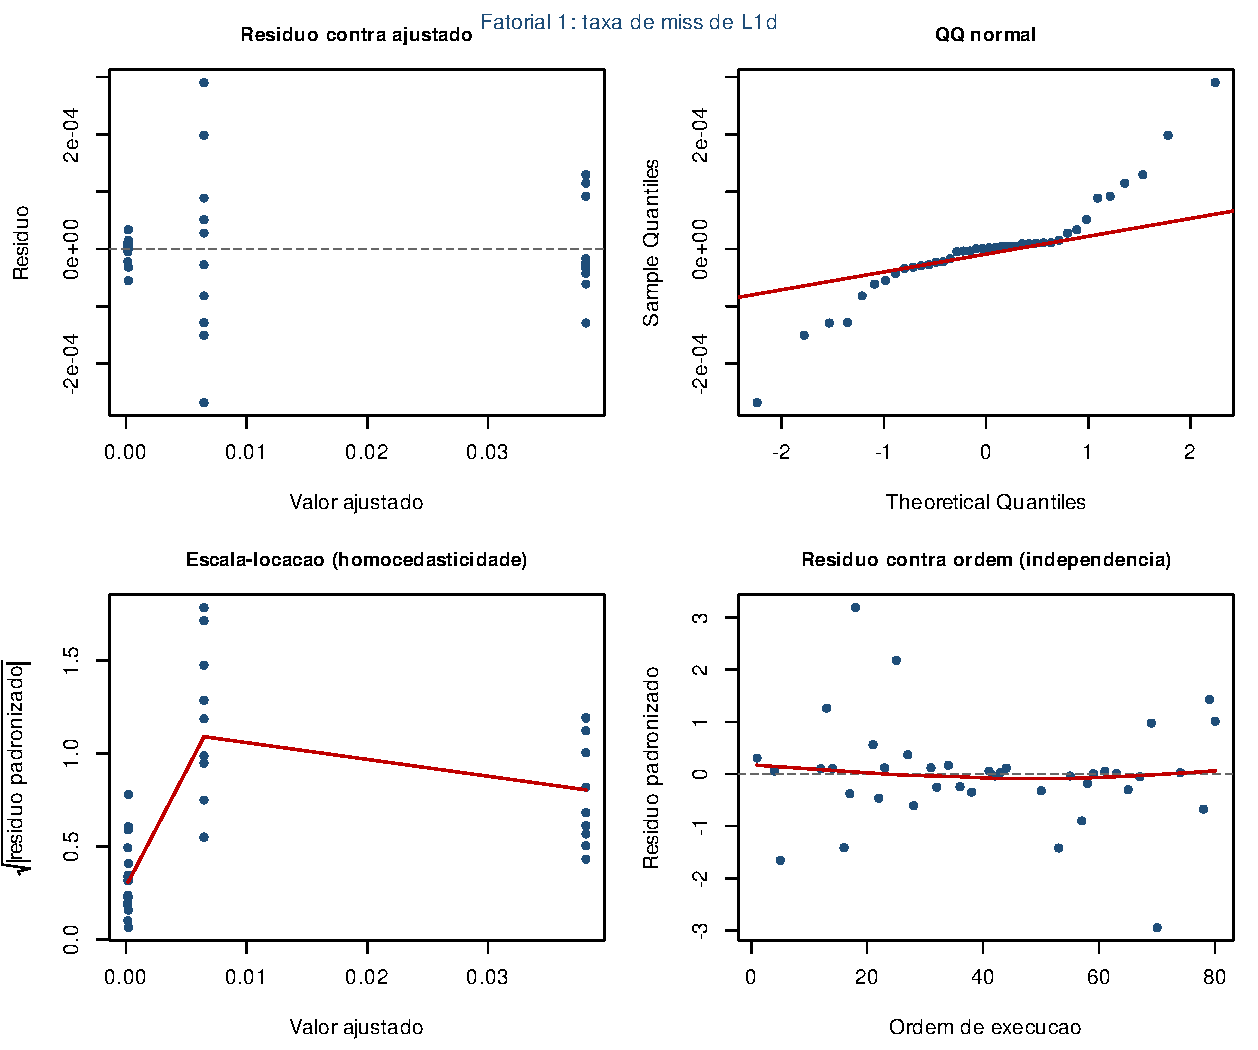
\includegraphics[width=0.88\textwidth]{figuras/residuos_fat1.pdf}
\caption{Diagnóstico de resíduos da análise de cache.}
\label{fig:res1}
\end{figure}

\begin{figure}[H]
\centering
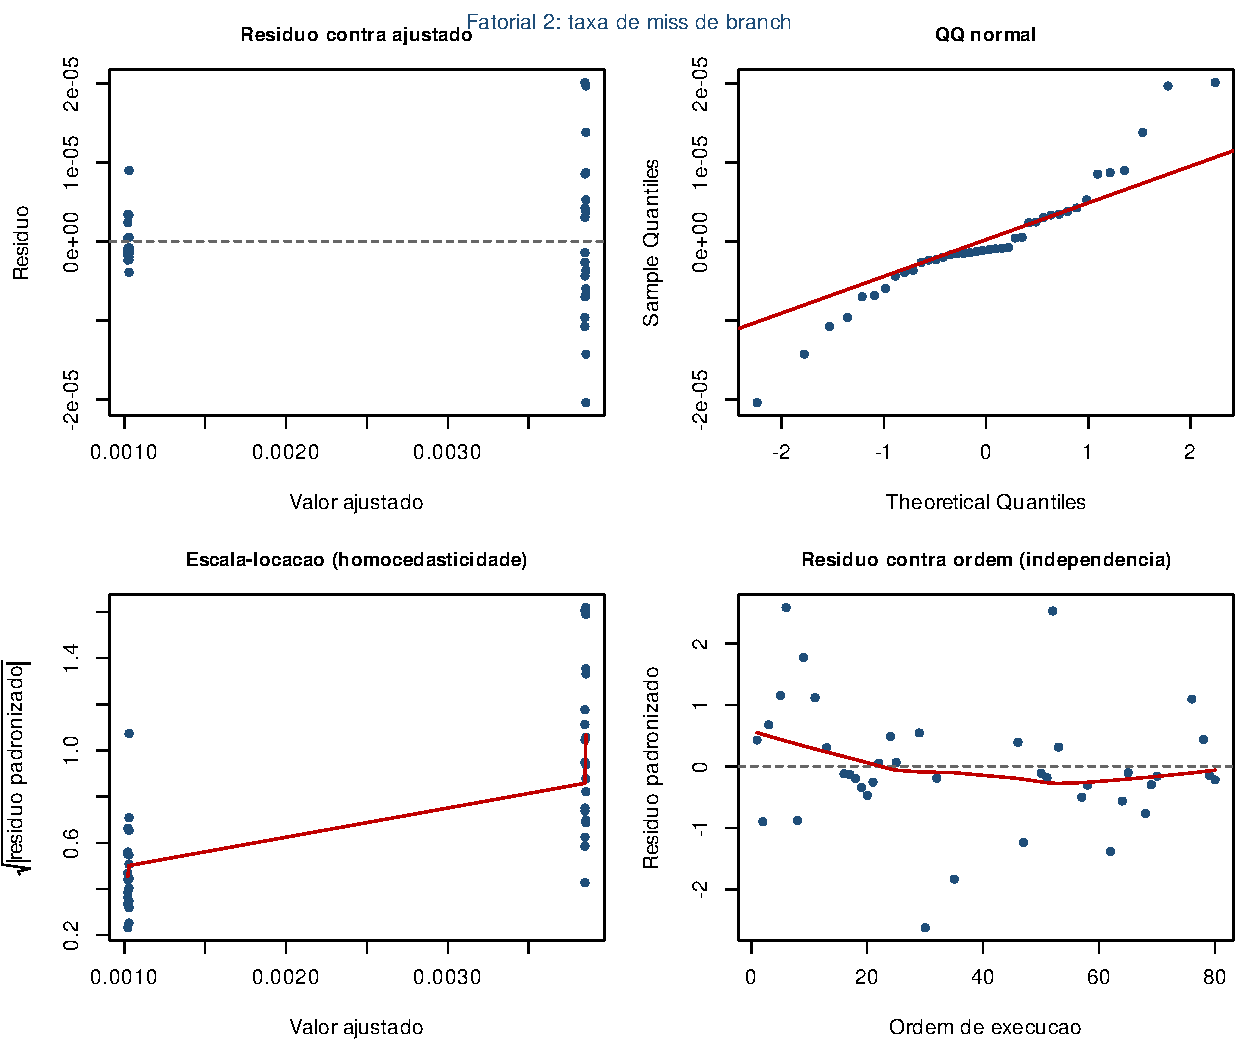
\includegraphics[width=0.88\textwidth]{figuras/residuos_fat2.pdf}
\caption{Diagnóstico de resíduos da análise de branch.}
\label{fig:res2}
\end{figure}

A concordância é total, \valFatUmPermConc{} de 3 efeitos na análise de cache e
\valFatDoisPermConc{} de 3 na de branch. Os valores de $p$ da permutação rastreiam de
perto os da análise de variância, inclusive no único efeito não significativo. O veredito
de significância, portanto, não depende do pressuposto de normalidade que foi rejeitado.


\end{document}
